\chapter{Stochastic Tractography}
\begin{figure} \label{fig:stflow}
	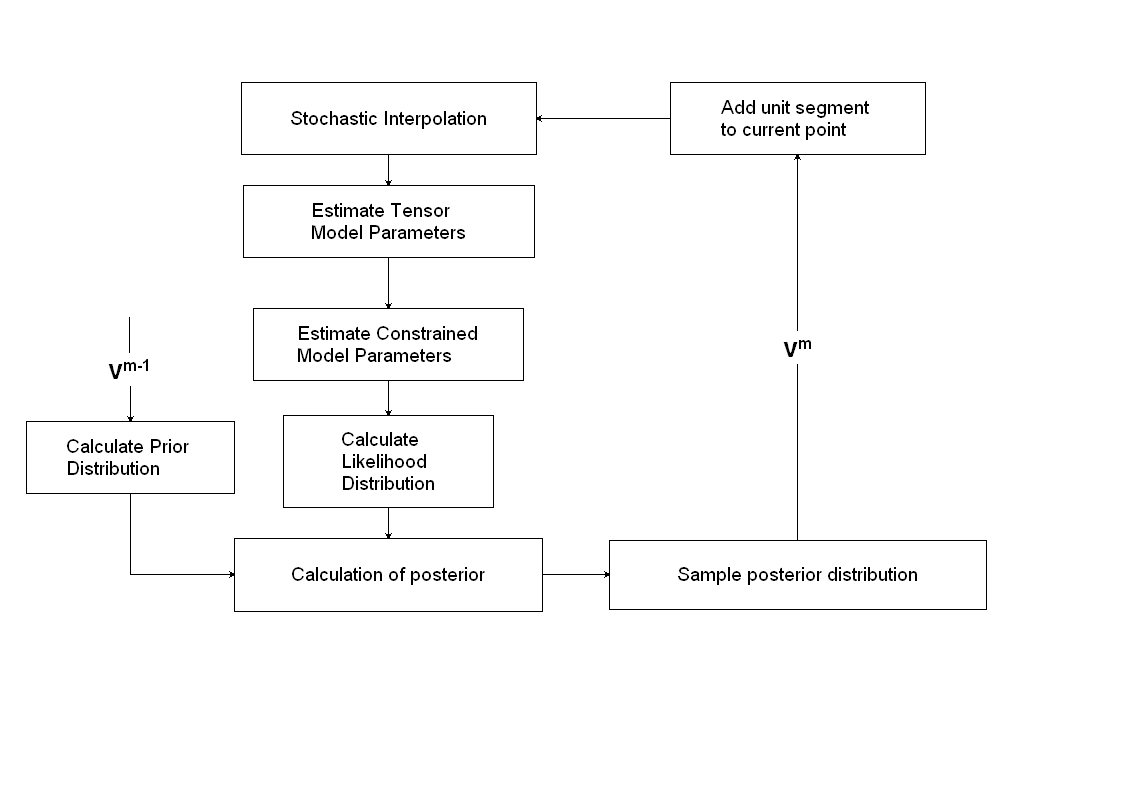
\includegraphics[width=\linewidth]{stflow}
	\caption{A flow chart demonstrating key steps in the stochastic tractgraphy algorithm}
\end{figure}
The Stochastic Tractography System implemented in this research implements Friman's \cite{frimanTMI06} approach to Stochastic Tractography with some modifications to the stopping criteria.

Friman's approach is a bayesian based inference algorithm similar to Behren's but with some optimizations to Behrens's approach \cite{frimanTMI06}.  In contrast with Behrens's two-compartment observation model, the model used by Friman is derived from the thoroughly studied tensor model of diffusion.  The tensor model of diffusion attempts describes diffusion in each voxel using a symmetric tensor.  The Friman model assumes the two smallest eigenvectors of diffusion tensor are equal, constraining the shape of the diffusion tensor to a "cigar-like" shape. 
%talk through key portions of the math
%present a block diagram of the algorithm
Friman's stochastic tractography algorithm \cite{frimanTMI06} operates at two levels.  At the local level, he presents a constrained model of diffusion that is describes the relationship between the DWI data and the likelihood of a fiber tract producing that data.  At a more global level, fiber tract orientation distributions are sampled across many voxels to infer the probability that two regions in the brain are connected by a fiber tract.  This distinct division is also found in Behrens's original work \cite{behrensMRM03} on probabilistic tractography.



%need to add in a bit about how they are different in the way they sample the PDF
The parametric approaches developed by Behrens and Friman are conceptually similar but differ mainly in their methods of arriving at the probability density function of the fiber orientation.  Their methods differ both in the model they use to describe the relationship between fiber orientation and the DWI data as well as the method they use to sample the fiber orientation probability density function resulting from the choice of model.  Whereas Behrens's directly models the fiber orientation, Friman's model is concerned with the diffusion profile and infers the fiber orientation from this profile.  Although Behrens's two-compartment model may be more conceptually sound, the advantage of using Friman's "constrained model" is its mathematical tractability.  The constrained model is able to fit every voxel within a matter of seconds whereas Behrens model takes a couple of hours \cite{frimanTMI06}.  Additionally Friman avoids using MCMC techniques by assuming that parameters other than the principle diffusion direction are constant within each voxel.  Friman further demonstrates that these mathematical simplifications have little effect on the resulting tractography.  This project will implement Friman's approach to probabilistic tractography.
%talk about how it differs from other algorithms
%talk about using incorporating the posterior probability of white matter
%talk about why we choose to segment the gray/white matter using b0 image instead of using diffusion information
